\chapter{Application: Standing}\label{chap:standing}
In this chapter, a controller that uses vertical motion for balance control is implemented in the momentum-based control framework and tested on NASA's Valkyrie \cite{radford2015valkyrie} humanoid robot. Push recovery is tested while the robot is standing. To measure the improvement in balance control, there is compared with a controller that uses a constant reference height. Additionally, an alternative test method is briefly presented using Boston Dynamics' Atlas humanoid robot.

\section{Method}
As the polynomial trajectories of the previous chapter are constraining the vertical acceleration, these are not used in application. Instead, a bang-bang control law for vertical acceleration is designed, similar to the bang-bang control law for the vertical force constrained capture positions in Section \ref{sec:verticalforce}.

The desired \ac{CMP} $\rcmpd$ of Equation \ref{eq:rcmpd} is constrained to be inside the support polygon and is assumed to coincide with a desired \ac{CoP} $\rcopd$. The \ac{CoM} height is initially controlled using the default \ac{CoM} height PD-control law of Equation \ref{eq:defaultheightcontrol}.  While the robot is standing, the control law controls to the default, nominal height:
\begin{equation}
\ddzd =k_p(z_0-z) - k_d\dot{z},
\end{equation}
where $\ddzd$ is the desired vertical acceleration. 

The bang-bang controller is activated when a worst-case event is met. This worst-case event can for example be noted if traditional balance strategies are saturated, which is for example the case if the \ac{CoP} is on the polygon edge. Because $\rcmpd$ is proportionally controlled to the \ac{ICP} error $\icpe$, the bang-bang controller is activated based when the $\icpe$ is larger than a minimum \ac{ICP} error threshold $\icpemin$. 

The first and the second acceleration `bang' of the vertical motion controller are jerk limited, unlike the controller for the vertical force constrained capture positions in Section \ref{sec:verticalforce}. Also, the duration of each `bang' is not predefined, but determined online. Determining the duration online, allows for more control of the vertical dynamics, as the current state can be constantly evaluated on violation of the maximum height constraint. A predefined duration as in Section \ref{sec:verticalforce} does not use any feedback and is strictly feedfoward. In relation to these differences in control design, the following parameters are used:
\begin{itemize}
	%\item $\alpha_{\icpe}^+$: Threshold to turn the controller on $|\icpe|>\alpha_{\icpe}^+$, which for example can be tuned to activate the controller when $\rcmpd$ is near the edge of the polygon. 
	%\item $\alpha_{\icpe}^-$: Threshold to turn the controller off $|\icpe|<\alpha_{\icpe}^-$, when the robot is back to stability.
	\item $\dddot{z}_{max}$: maximum allowed vertical CoM jerk;
	\item $\alpha_{\hat{\ddot{z}}_{c}}$: parameter to scale down expected $\ddot{z}_c$ for the second `bang', due to jerk limits.
\end{itemize}
The control sequence for the vertical motion controller reads as follows. For the first `bang': the desired acceleration $\ddot{z}_d=\ddot{z}_c$. The transition from the first `bang' to the second is if the predicted \ac{CoM} height violates the height constraint. This prediction is computed as follows, in the case of approaching a maximum height constraint:
\begin{align}
	m\hat{g}z + \sgn(\dot{z})\frac{1}{2}\dot{z}^2>m\hat{g}\zmax,\\
	z + \sgn(\dot{z})\frac{1}{2}\frac{\dot{z}^2}{\hat{g}}>\zmax,
\end{align}
where $\hat{g}$ is the predicted gravity, or the predicted \textit{downward acceleration}. Using the acceleration constant $\ddzc$ of the second bang, and the scale down parameter $\alpha_{\hat{\ddot{z}}_{c}}$, gives:
\begin{equation}
	z+\sgn(\dot{z})\frac{1}{2}\frac{\dot{z}^2}{\alpha_{\hat{\ddot{z}}_{c}}\ddot{z}_{c}} >\zmax.
\end{equation}
When this condition is met, the second `bang' is activated and $\ddot{z}_d=-\ddot{z}_c$. The second `bang' continues until the vertical velocity changes direction: $\dot{z}<0$. This results in the height to be controlled to $\zmax$ until the controller turns off:
\begin{equation}
	\ddot{z}_d = k_p(\zmax-z)-k_d\dot{z}.
\end{equation}
Controlling to $\zmax$ allows the robot to apply more force on the ground, compared to controlling directly to $z_0$ again. The controller turns off if the \ac{ICP} error $\icpe$ is at a small value, a measure for stability. If the controller is turned off, the height is controlled to the default height and reference height $z_r=z_0$. Finally, the rate of $\ddot{z}_d$ is limited with the maximum allowed jerk and the desired vertical momentum rate is computed as $\dot{\mathbf{l}}_{d,z}=m\ddot{z}_d$. The desired horizontal linear momentum rate is adjusted for the added vertical acceleration as follows:
\begin{equation}
    \dotldxy= \frac{\cxy-\rcmpd}{z_0}(mg+\dot{\mathbf{l}}_{d,z}).
\end{equation}

\section{Results}
Tests are conducted by applying a push at chest height on Valkyrie. The parameters and settings used for the tests can be found in Appendix \ref{chap:params}. Additionally, some tests are conducted on Atlas.

\subsection{Simulation}
In simulation the push duration is set to $\tpush=0.15$ [s], as on hardware tests is found that approximately the same push duration can be applied. The push force profile in simulation is constant. A vertical acceleration constant of $\ddzc=2.4$ [m/s$^2$] is used, as this was also found to work well on hardware. A value of $\alpha_{\hat{\ddot{z}}_{c}}=0.4$ was used for the prediction of vertical motion.

\paragraph{The maximum recoverable impulses} for the vertical motion controller and the default controller setup are shown in \figref{fig:roundStanding}. The results are obtained with a search for the maximum push that the robot could still recover from. This search is conducted every $5$ degrees. The radius of the plot is the normalized impulse $i$ applied to the robot:
\begin{equation}
	i = \frac{\int \fpush d\tpush}{\mrobot},
\end{equation}
where $\fpush$ is the push force and $\mrobot$ the robot mass. Valkyrie has a total mass of $\mrobot=127.3$.

The recovery improved after using the vertical motion controller in push directions coming from the back or the side of the robot. Remarkably, push recovery is worse for push directions coming from the front of the robot. Compared to the default setup, the vertical motion controller recovered of a $9$\% higher impulse for a push direction coming from the back of the robot, $4$\% for a push direction coming from the side and $-7$\% for a push direction coming from the front. The improvement in maximum recoverable push is the best for a push coming from the back. Also, it is relatively easy to apply a push in the back on the real robot, compared to other parts of the robot. Valkyrie has a hard, flat back surface, which can handle larger impacts than other body parts. For those reasons, there is chosen to make a deeper evaluation of the specific push direction of $0$ degrees in simulation too.
\begin{figure}
\centering
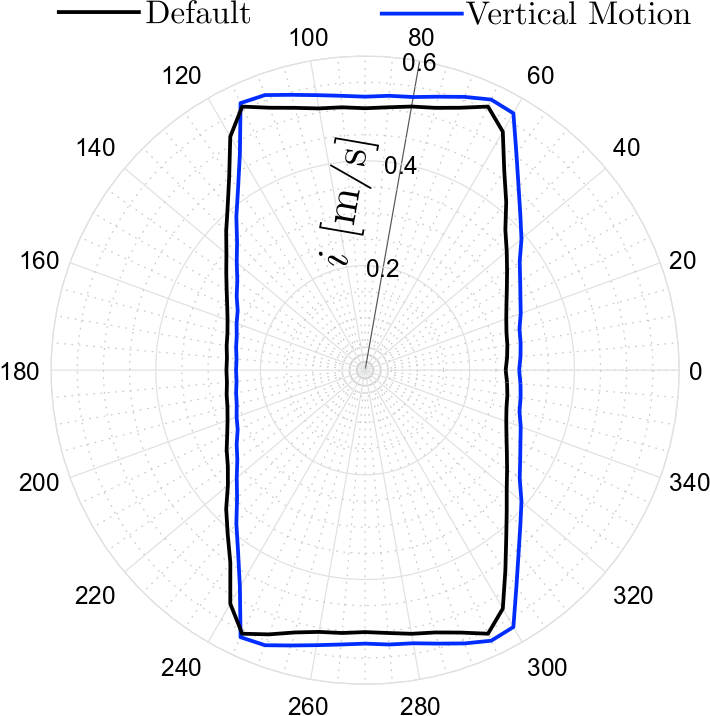
\includegraphics[width=0.6\textwidth]{STYLESTUFF/roundStanding.png}
\caption{Polar plot of maximum recoverable pushes with an increment of $5$ degrees. $0$ degrees is a push from the back. The radius is the normalized impulse $i$. }
\label{fig:roundStanding}
\end{figure}

\paragraph{Comparison of the response after equal push magnitudes} is shown in \figref{fig:valcomparephase}, as a phase plot for the horizontal \ac{CoM} state in the sagittal plane. The area covered by the phase plot is smaller with the vertical motion controller for a push of $i=0.271$ [m/s]. With the larger push of $i=0.295$ [m/s], the default control setup does not manage to stabilize and diverges, while the vertical motion controlled setup recovers.
\begin{figure}
\centering
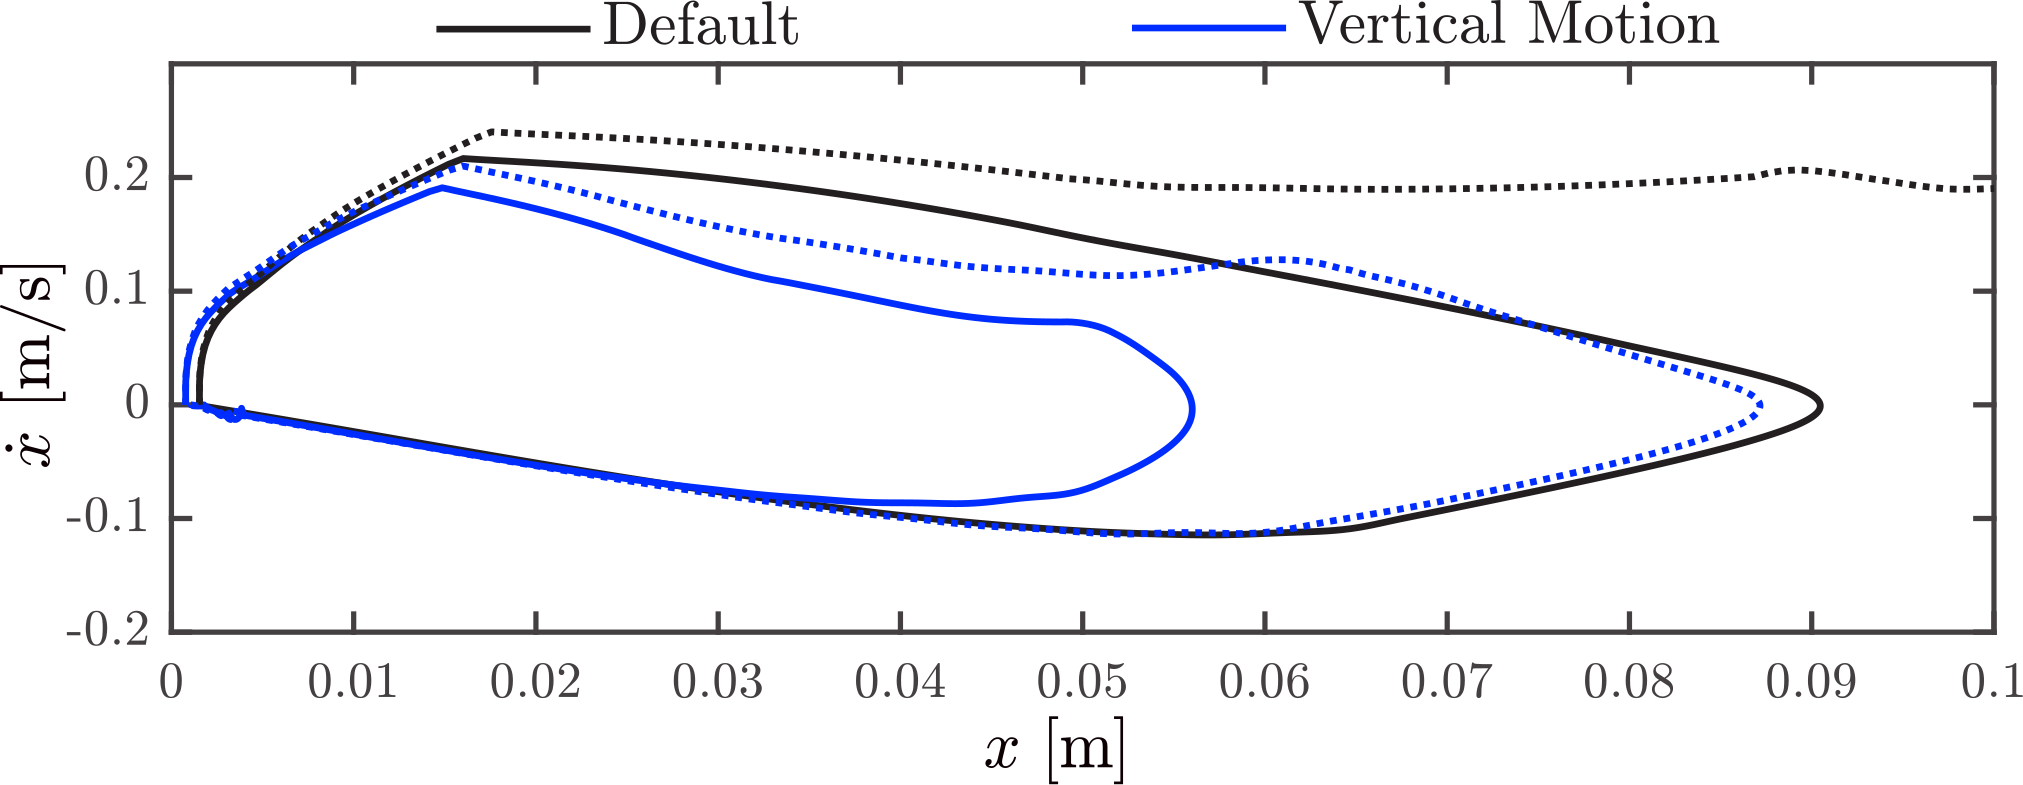
\includegraphics[width=0.9\textwidth]{STYLESTUFF/valcomparephase.png}
\caption{Phase plot of horitzontal \ac{CoM} motion in the sagittal plane for a push of $i=0.271$ [m/s] (solid) and a push of $i=0.295$ [m/s] (dotted).}
\label{fig:valcomparephase}
\end{figure}

In \figref{fig:valcomparetime}, time response plots are shown for a push of $i=0.271$ [m/s]. `Achieved' is the value after the \ac{QP} found a solution. For the vertical linear momentum rate $\dot{\mathbf{l}}_z$, the achieved tracks the desired fairly well. There is a larger difference between the desired and achieved horizontal linear momentum rate $\dot{\mathbf{l}}_x$ for both control setups. If the achieved is compared between the two setups, the vertical motion controller achieves almost double the amount the default control setup achieves from $0.1$ [s] until $0.25$ [s]. There is a small difference in achieved angular momentum rate observable. However, if there is looked at the pelvis error $\theta_{pel,y}$ and the torso error $\theta_{torso,y}$ in the fifth and sixth row, the vertical motion controller has even a little less rotation error than the default setup. 
\begin{figure}
\centering
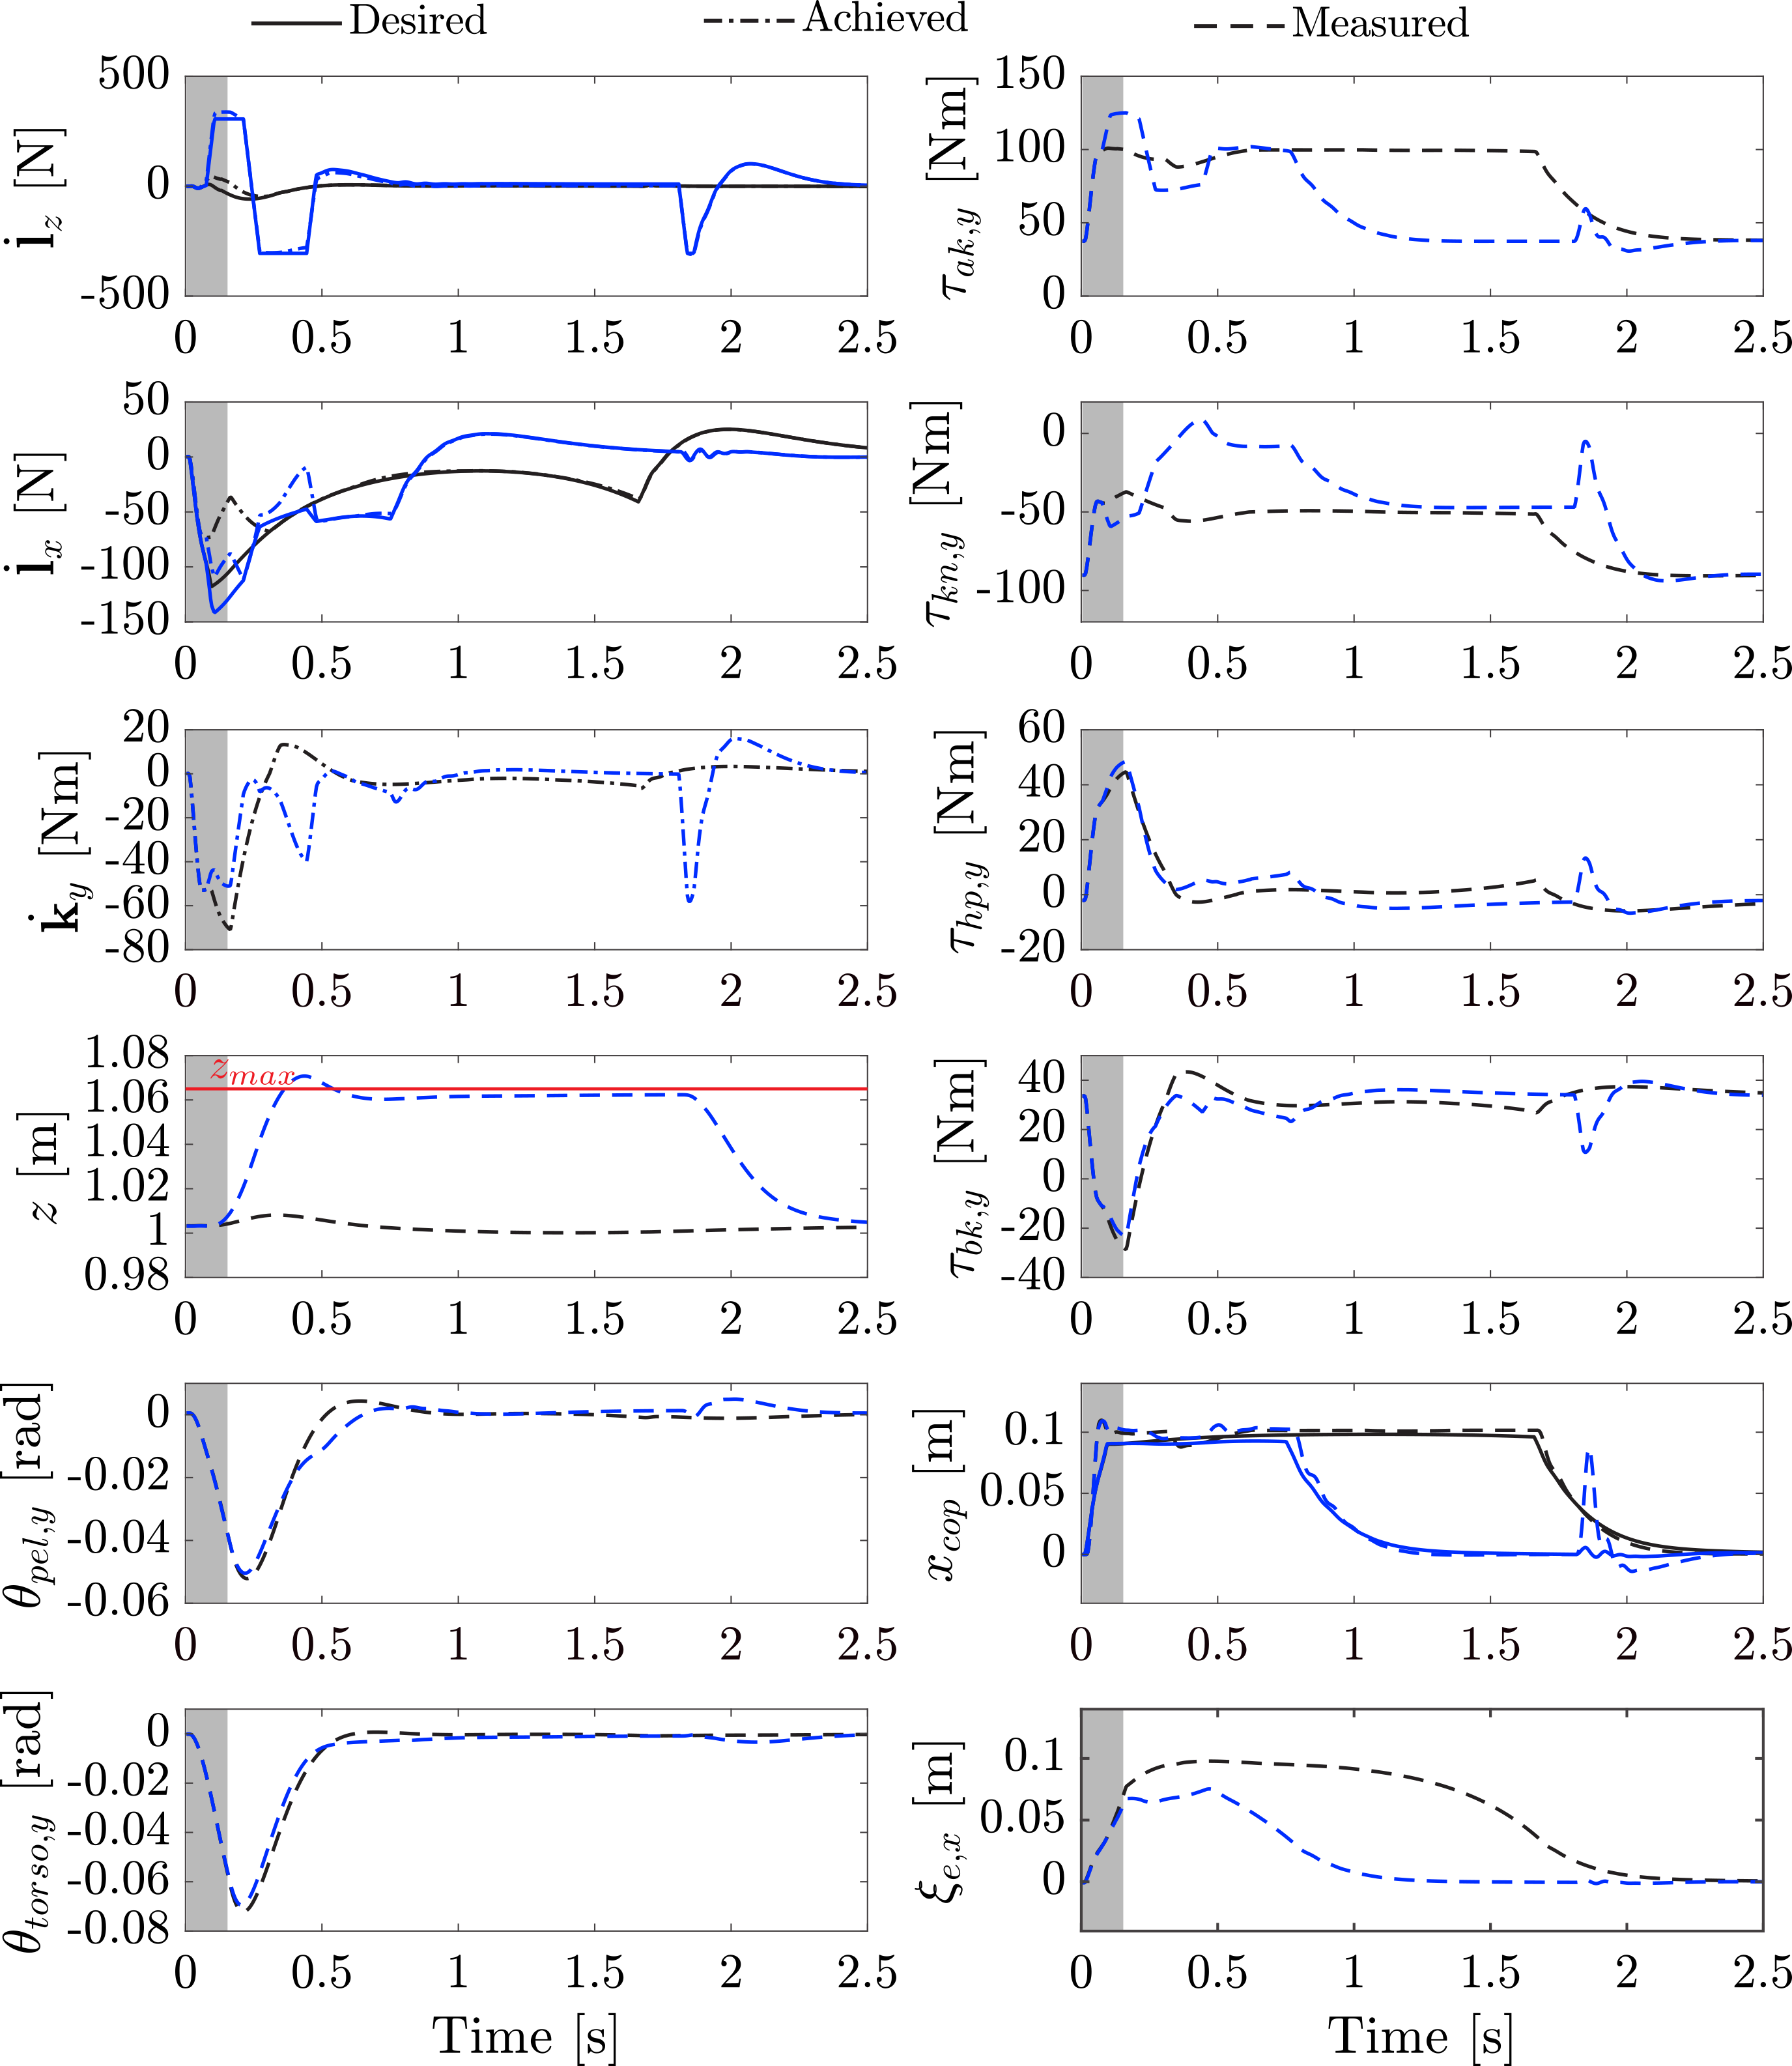
\includegraphics[width=1.0\textwidth]{STYLESTUFF/valcomparetime.png}
\caption{Time plots for a push of $i=0.271$ [m/s]. `Achieved' is the value of the variable after the \ac{QP} found a solution. The gray area is where the push is applied.}
\label{fig:valcomparetime}
\end{figure}

In the right column of the figure, from the ankle torque $\tau_{ak,y}$, knee torque ankle torque $\tau_{kn,y}$, hip torque $\tau_{hp,y}$ and back torque $\tau_{bk,y}$, the difference in ankle and knee torque is the most noteworthy. The ankle torque has a higher peak for the vertical motion controller. Also, the ankle torque returns to the steady state value earlier than the default control setup. Equivalently, the desired and measured \ac{CoP} returns to the steady state value earlier as well. This is an indication of a slight increase in robustness for the push, as is observed in the phase plot as well. The knee torque is on average lower for the vertical motion controller. On average, the \ac{ICP} error $\xi_{e,x}$ is smaller, as expected.

\subsection{Hardware} 
Hardware tests are conducted by applying a push in the back at chest height on the physical robot. An iLoad Pro Digital load censor \cite{iload} is used to measure the impulse of the push. The load sensor is mounted to a aluminum stick. On the other end of the load cell, a steel plate with a rubber surface is mounted. This prevents the robot from being damaged, and makes the push data less dependent on contact impacts. In \figref{fig:pushhead}, the end of the push stick with the load sensor is depicted. In \figref{fig:authorpush}, the test setup is shown. A value of $\alpha_{\hat{\ddot{z}}_{c}}=0.8$ is used for the prediction of the vertical dynamics. 
\begin{figure}
\centering
  \begin{subfigure}{0.495\textwidth}
  \centering
  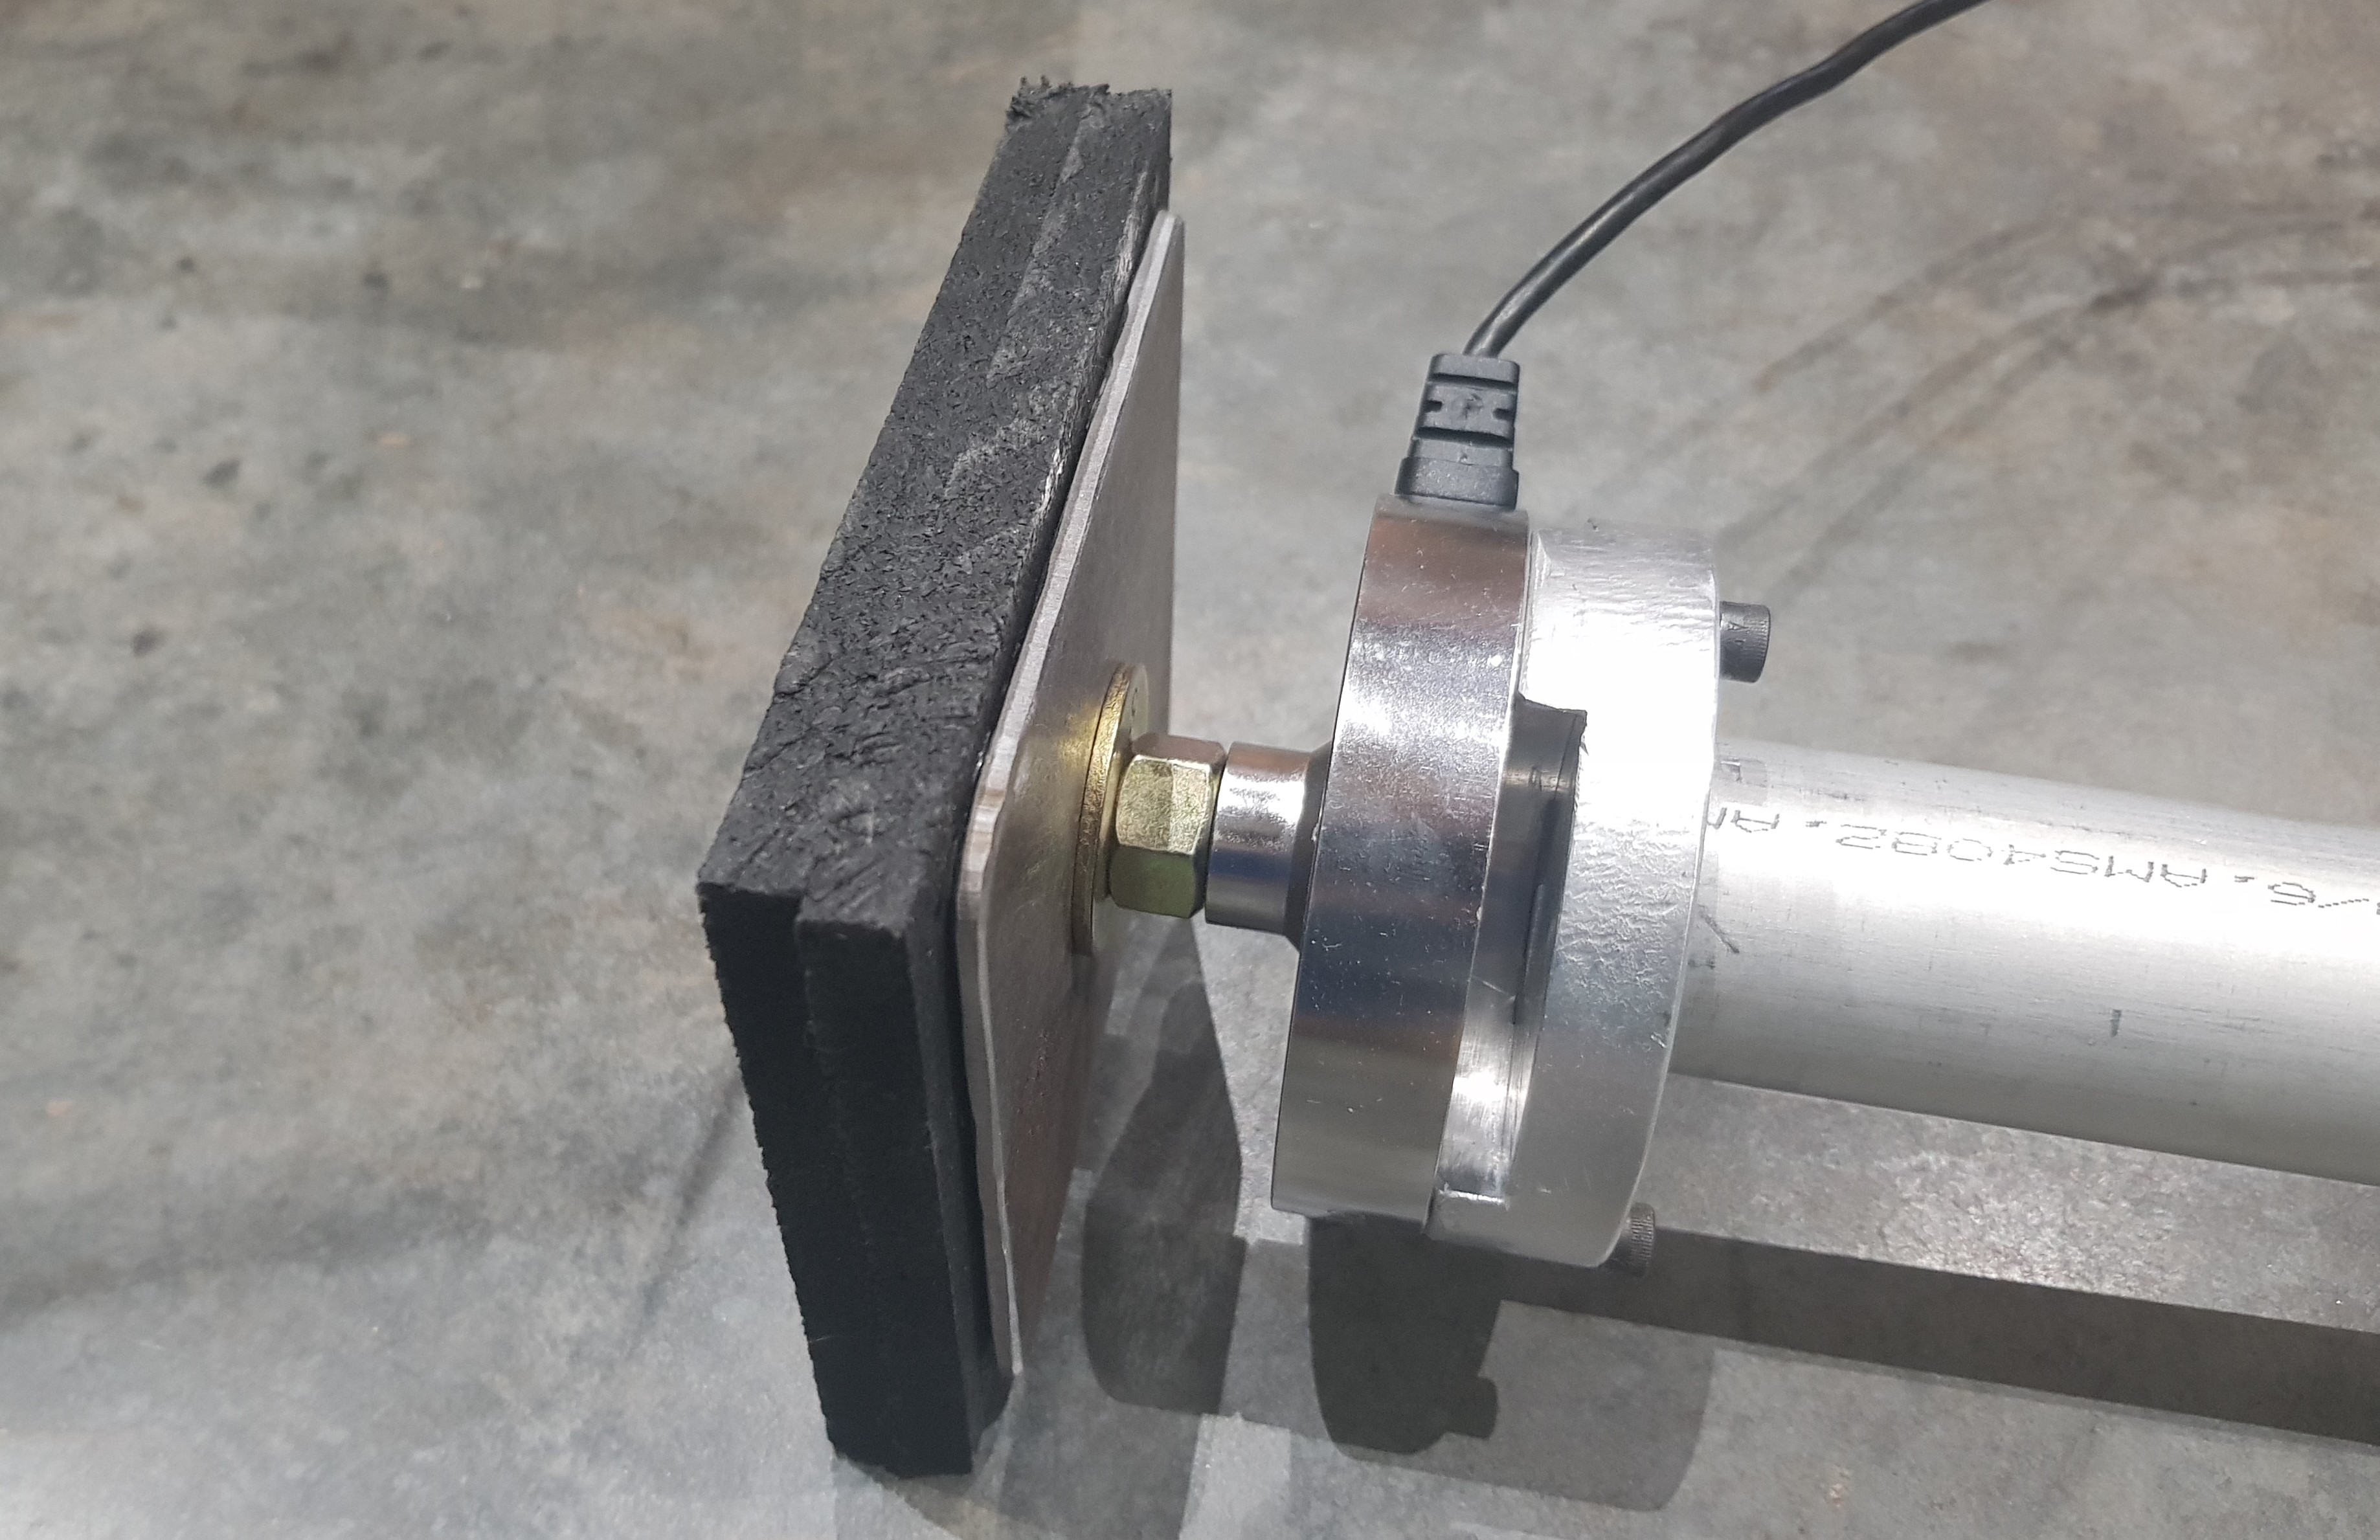
\includegraphics[width=.94\linewidth]{STYLESTUFF/pushhead.png}
   \caption{}
    \label{fig:pushhead}
  \end{subfigure}
  \begin{subfigure}{0.495\textwidth}
    \centering
  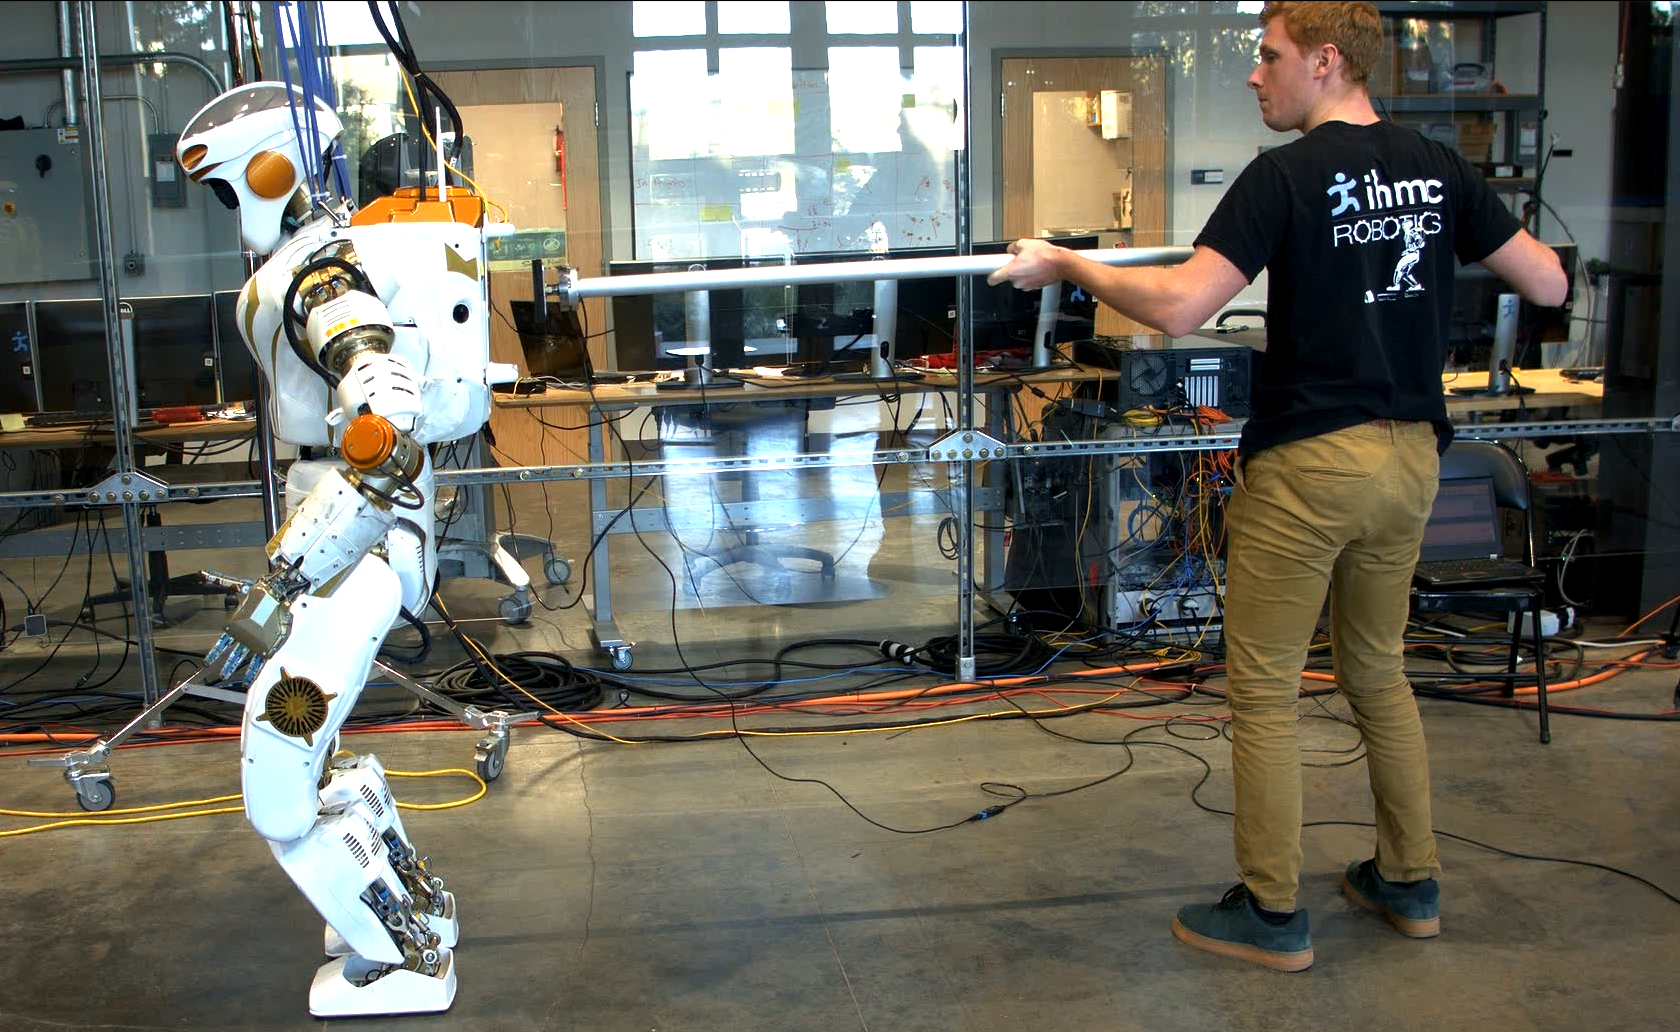
\includegraphics[width=.94\linewidth]{STYLESTUFF/authorpush.png}
  \caption{}
   \label{fig:authorpush}
  \end{subfigure}
  \caption{(a) Push head of push stick with the rubber surface, steel plate, load sensor and aluminum stick. (b) Tests setup, where the author applies a push using the push stick on Valkyrie.}
  \label{fig:pushsetup}
\end{figure}

\paragraph{The maximum recoverable push} is determined by averaging a dozen cases, where the \ac{CoM} of the robot came closer than $5$ [mm] from the polygon edge, but the robot still recovered. In \figref{fig:imp1}, the average force profile with the standard deviation of the $12$ pushes is depicted for the default setup. The average impulse is $35.3$ [Ns], which equals a normalized impulse of $i=\frac{35.3}{127.3}=0.277$ [m/s]. This is a slightly higher value than the impulse recoverable in simulation. In \figref{fig:imp2}, the average force profile with the standard deviation is depicted for the vertical motion controller. The average impulse is $37.6$ [Ns], which equals $i=0.295$ [m/s], which is an increase in recoverable push of approximately $7$\%.
\begin{figure}
\centering
  \begin{subfigure}{0.32\textwidth}
  \centering
  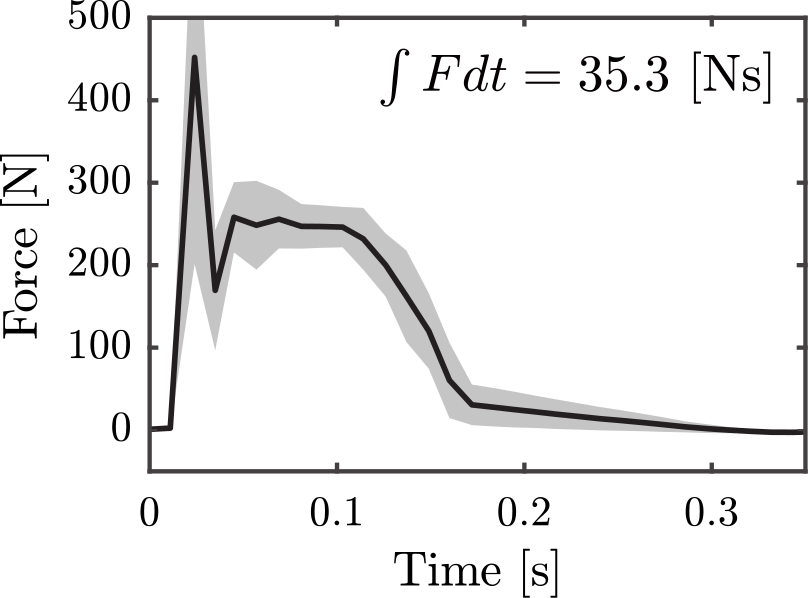
\includegraphics[width=.9\linewidth]{STYLESTUFF/impulsecompare1.png}
   \caption{}
    \label{fig:imp1}
  \end{subfigure}
    \begin{subfigure}{0.32\textwidth}
  \centering
  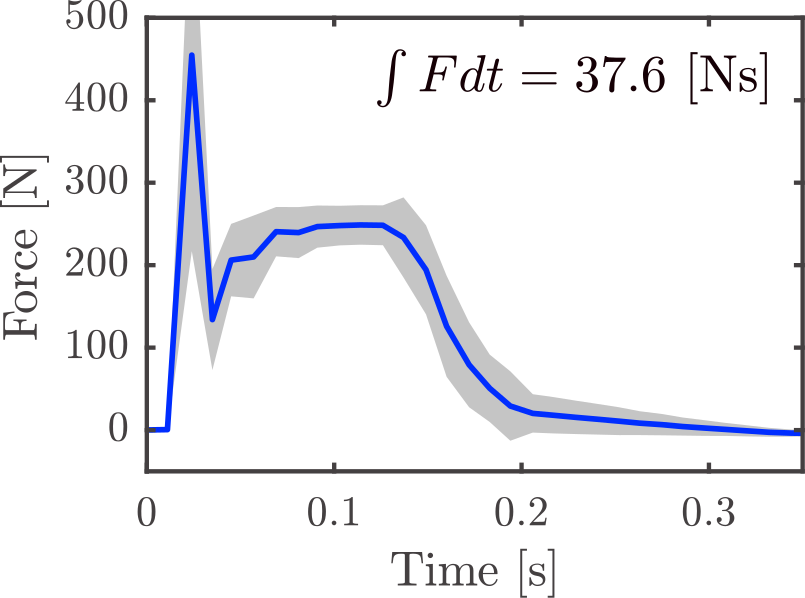
\includegraphics[width=.9\linewidth]{STYLESTUFF/impulsecompare2.png}
   \caption{}
    \label{fig:imp2}
  \end{subfigure}
  \begin{subfigure}{0.32\textwidth}
    \centering
  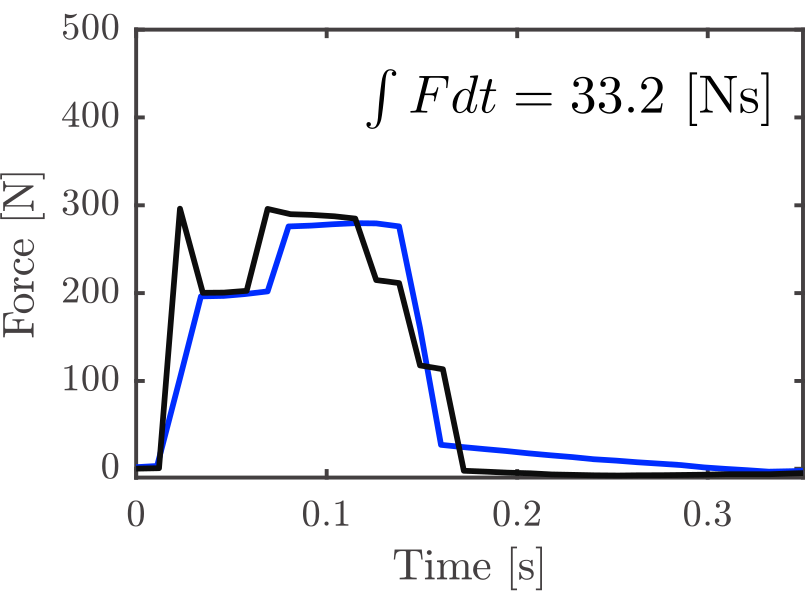
\includegraphics[width=.9\linewidth]{STYLESTUFF/impulsecompare3.png}
  \caption{}
   \label{fig:imp3}
  \end{subfigure}
  \caption{Average impulse of $12$ pushes, where the \ac{CoM} came closer than $5$ [mm] from the polygon edge for the (a) default setup and (b) vertical motion controller. (c) Two picks of pushes, where the force profile and integrated force applied on both setups were approximately equal. }
  \label{fig:impulsecompare}
\end{figure}

\begin{figure}
\centering
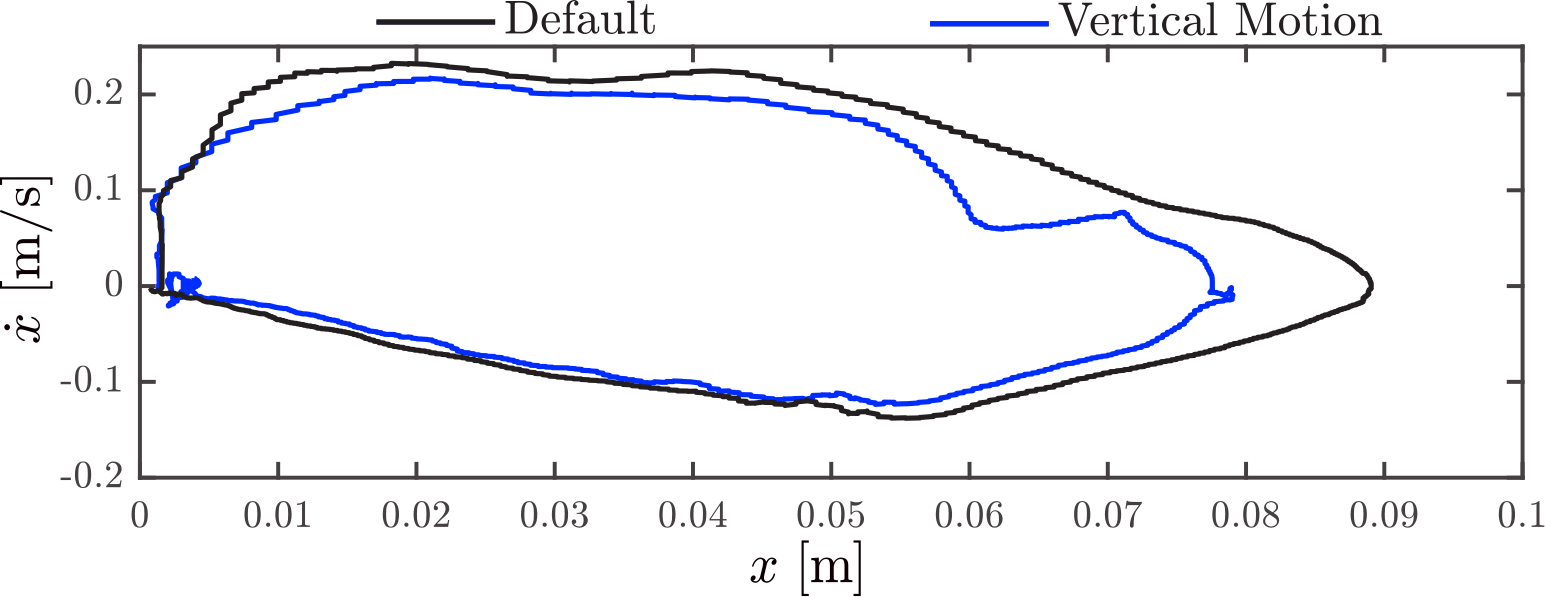
\includegraphics[width=0.7\textwidth]{STYLESTUFF/valcomparephaseHW.png}
\caption{Phase plot of forward \ac{CoM} motion for a push of $i=0.261$ [m/s].}
\label{fig:valcomparephaseHW}
\end{figure}
\begin{figure}
\centering
  \begin{tabular}{ccccccc}
    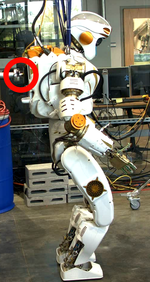
\includegraphics[width=0.7in]{STYLESTUFF/val1zr_C} &
    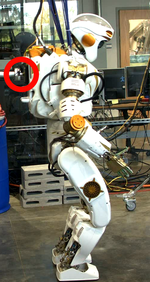
\includegraphics[width=0.7in]{STYLESTUFF/val2zr_30} &
    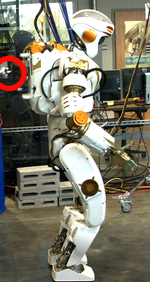
\includegraphics[width=0.7in]{STYLESTUFF/val3zr_30} &
    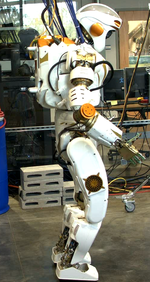
\includegraphics[width=0.7in]{STYLESTUFF/val4z_30} &
    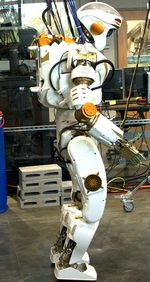
\includegraphics[width=0.7in]{STYLESTUFF/val5z_30} &
    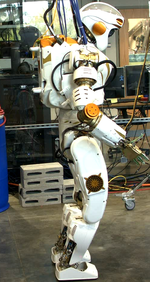
\includegraphics[width=0.7in]{STYLESTUFF/val6z_30} &
    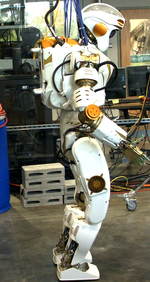
\includegraphics[width=0.7in]{STYLESTUFF/val7z_30} ~\\[2ex]
     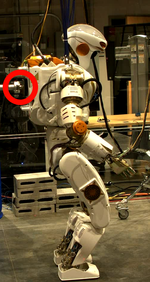
\includegraphics[width=0.7in]{STYLESTUFF/val1dr_C} &
    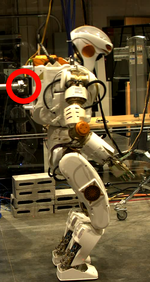
\includegraphics[width=0.7in]{STYLESTUFF/val2dr_30} &
    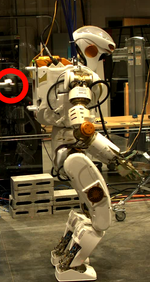
\includegraphics[width=0.7in]{STYLESTUFF/val3dr_30} &
    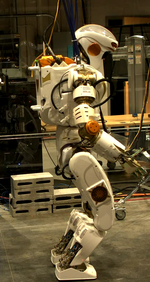
\includegraphics[width=0.7in]{STYLESTUFF/val4d_30} &
    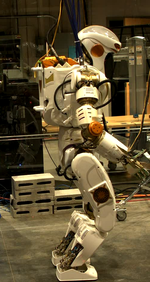
\includegraphics[width=0.7in]{STYLESTUFF/val5d_30} &
    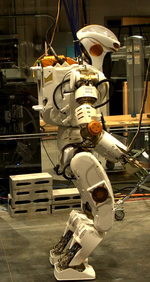
\includegraphics[width=0.7in]{STYLESTUFF/val6d_30} &
    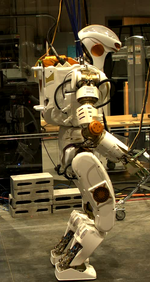
\includegraphics[width=0.7in]{STYLESTUFF/val7d_30} \\
    $a$&
    $b$&
    $c$&
    $d$&
    $e$&
    $f$&
    $g$\\
  \end{tabular}
  \caption{Time-lapse of Valkyrie recovering from a push using vertical motion (top row) and using the default controller setup (bottom row). The letters below the columns match with the letters next to the yellow lines in Figure \ref{fig:valcomparetimeHW}. The push rod tip is encircled in red.}
  \label{fig:val}
\end{figure}

\paragraph{Comparison of the response after equal push magnitudes} is conducted by selecting a force profile from each setup, where the integrated force is approximately equal and the force profiles had a comparable shape. In \figref{fig:imp3}, the two compared force profiles are shown and have an impulse of $33.2$ [Ns], which is equal to $i=0.261$ [m/s]. In \figref{fig:valcomparephaseHW}, a phase plot for the sagittal horizontal motion is depicted. Again, the vertical motion covers a smaller area. 

In \figref{fig:val}, a time-lapse is shown for both control setups after these pushes. The letters under each column match with the letters next to the vertical lines in \figref{fig:valcomparetimeHW}. In \figref{fig:valcomparetimeHW}, time response plots are shown for the pushes of $i=0.261$ [m/s]. Note how the vertical lines leave the gray area, when in the \figref{fig:val} the red encircled push head loses contact with the robot. 
\begin{figure}
\centering
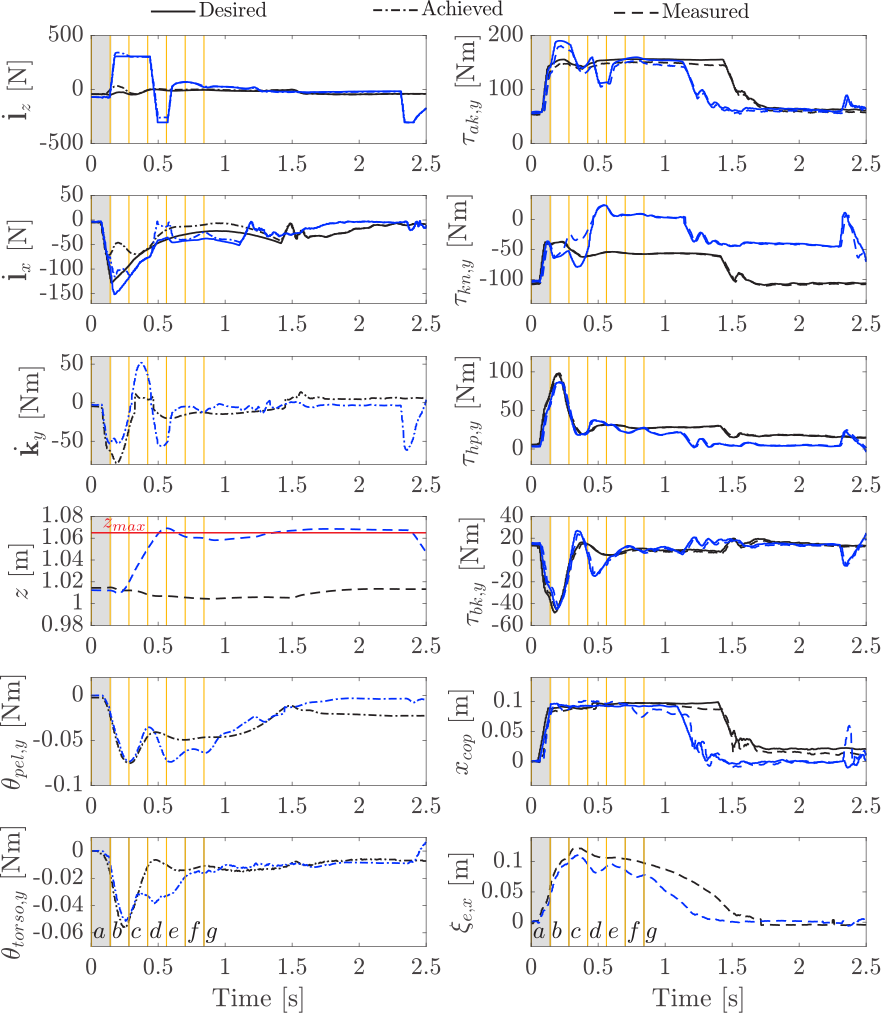
\includegraphics[width=1.0\textwidth]{STYLESTUFF/valcomparetimeHW.png}
\caption{Time plots for a push of $i=0.261$ [m/s]. All joint torques, except for the back, are the average over left and right.}
\label{fig:valcomparetimeHW}
\end{figure}

Also note how each `bang', visible in the vertical linear momentum rate $\dot{\mathbf{l}}_z$, has a relatively a different length compared to the results observed in simulation. This might be a reason why are larger value of $\alpha_{\hat{\ddot{z}}_{c}}$ could be used. The $\dot{\mathbf{l}}_x$ plots are comparable with the simulation results. The achieved $\dot{\mathbf{k}}_y$ of the vertical motion controller has a relatively larger overshoot than in simulation. However, the resulting pelvis and torso rotation errors are not larger for the vertical motion controller compared to the default setup, which does shows no additional use of `hip' strategies. 

In the right column of the figure, the torques have a desired and a measured value, as the torques of the robot are PD-controlled with electrical current as input. Again, the difference in ankle torque between the default setup and the vertical motion controller is the most noteworthy. For the vertical motion controller, the ankle torque returns quicker to steady state, just like the \ac{CoP}, which shows a slight increase in robustness for the applied push. Equivalently, the average \ac{ICP} error is again smaller for the vertical motion controller.

\subsection{Comparison with Capture Regions}
On all tests, the time until the \ac{ICP} error turns, can be seen as the part that is crucial for recovery, as the \ac{ICP} error would not turn and diverge if the robot falls over. If in this crucial part the assumption is made that the \ac{CoP} is at a constant location and the impulse $i$ is an instant impulse, a comparison can be made with the capturability comparison in Section \ref{sec:capcomparenoinertia}. Also, the assumption is made that the difference in recovery between the default setup and the vertical motion controller is comparable with the difference between the \ac{CP} and the vertical force constrained capture position of Section \ref{sec:verticalforce} for the same $\ddzc$.

Considering the assumptions mentioned above, in \figref{fig:regioncomparison}, the differences in recovery for the experiments are plotted in the capture velocity graph of \figref{fig:capcompare} in Section \ref{sec:capcomparenoinertia}. Note that the point $[1,1]$ in the plot corresponds to either the \ac{CP}, or the recovery of the default setup for the corresponding push direction. The dimensionless acceleration $\ddzc'=\frac{1}{4}$ roughly corresponds with the value of $\ddzc=2.4$ [m/s$^2$] used on the experiments on Valkyrie. 
\begin{figure}
\centering
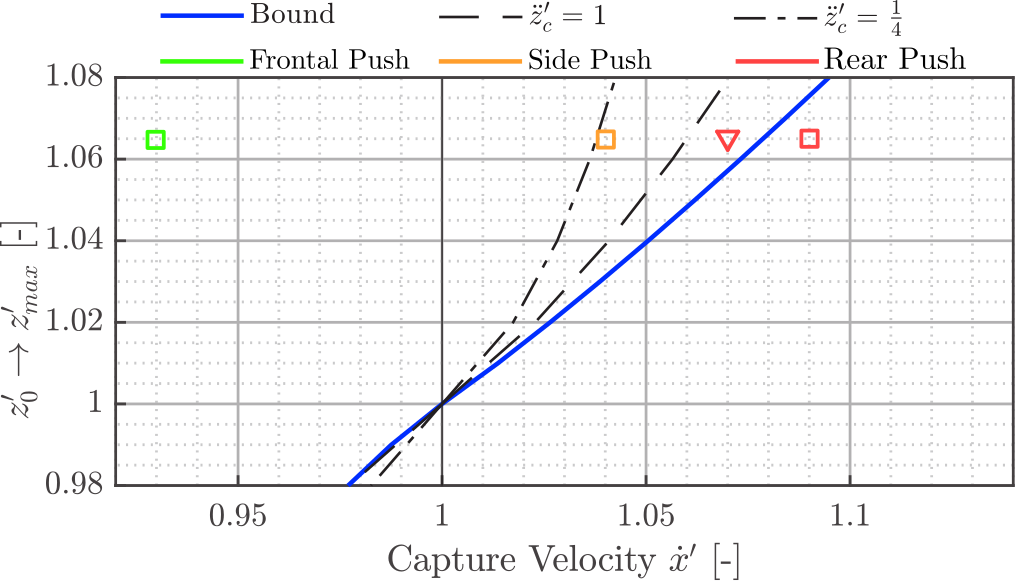
\includegraphics[width=0.9\textwidth]{STYLESTUFF/regioncomparison.png}
\caption{Difference in recovery of Valkyrie in simulation (rectangle) and on hardware (triangle) between the vertical motion controller and the default setup versus the capture velocity plot of Section \ref{sec:capcomparenoinertia}.}
\label{fig:regioncomparison}
\end{figure}

Note how the simulation rear push recovery even lies outside the height constrained bound in this plot. The average improvement on hardware lies just inside the height constrained bound. The side push recovers about equal to the comparable force constrained capture position of $\ddzc'=\frac{1}{4}$. The frontal push recovers worse than the default control setup and is not comparable with the capture regions presented in Chapter \ref{chap:regions}.

\subsection{Atlas Results}
Next to the Valkyrie tests, some tests are conducted on Boston Dynamics' Atlas humanoid robot. An alternative experimental setup is used to test push recovery on hardware. A medicine ball with mass $m_{ball}=13.6$ [kg] is hung from the ceiling at the robotics lab of \ac{IHMC}. To push the robot, the ball can be released from a certain distance, where the impulse on the robot is assumed to be only depending on the difference in potential energy of the ball. To protect the robot from the impact of the ball, a wooden plate is mounted to the frame. In \figref{fig:atlassetup}, the test setup is depicted. The length from the horizontal ball position to the dead point of the pendulum $\lball$ can be used to calculate the impulse applied on the robot. 
\begin{figure}
\centering
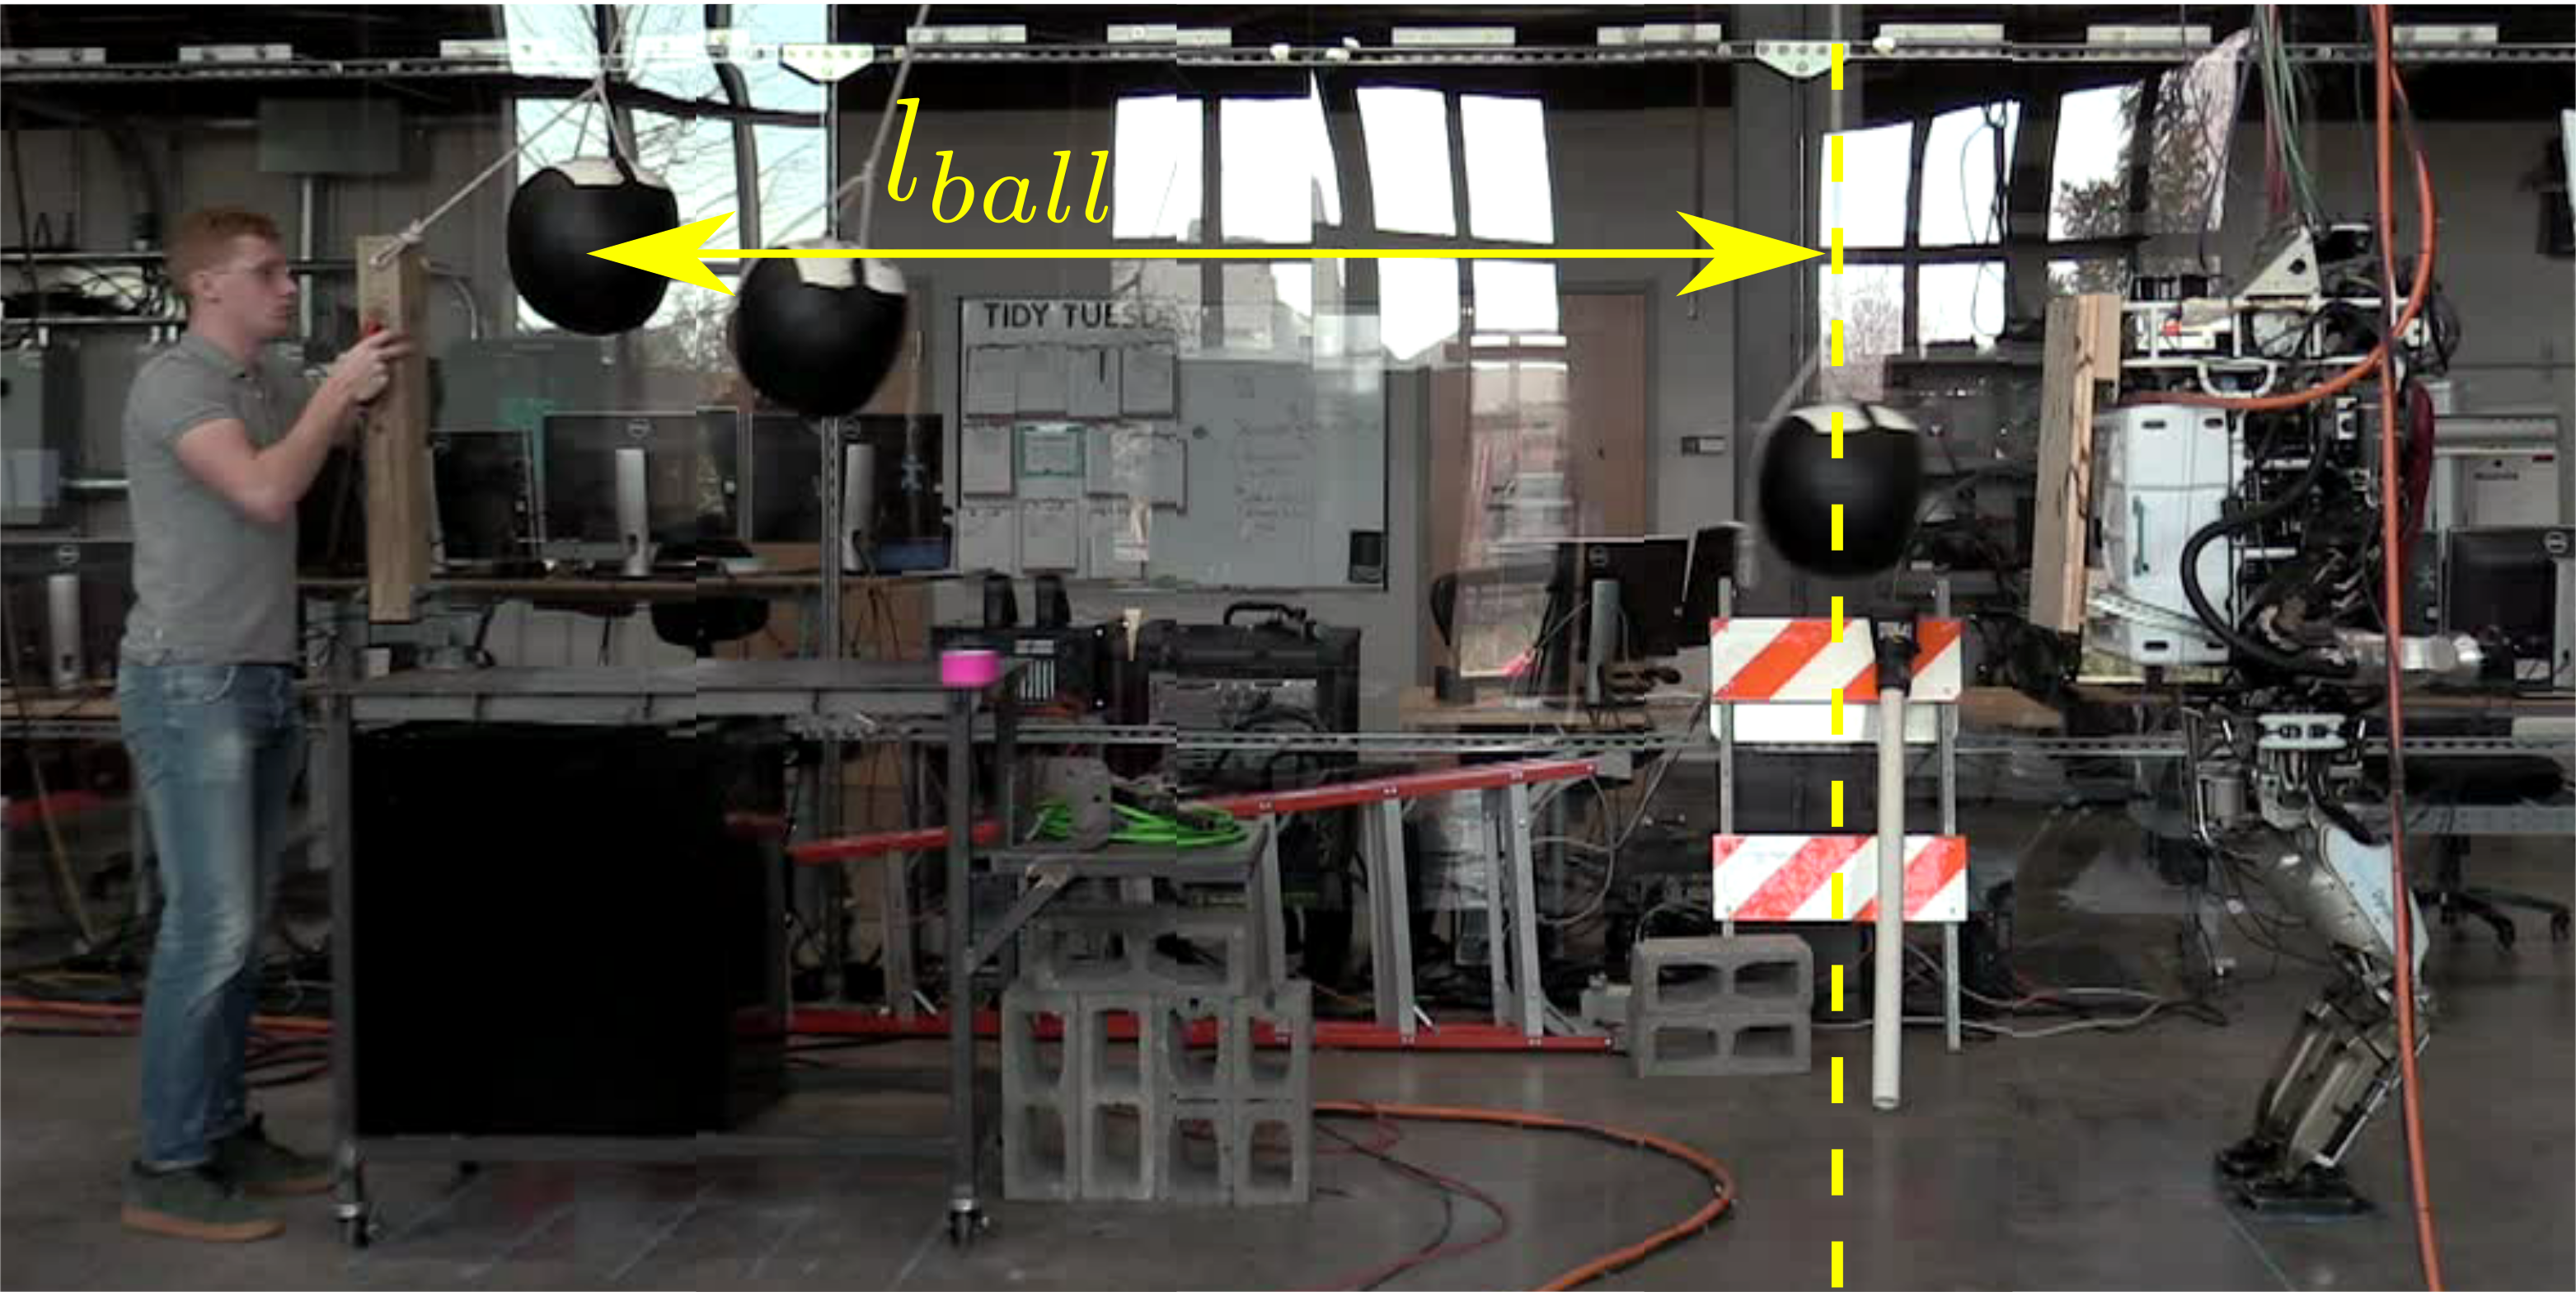
\includegraphics[width=0.99\textwidth]{STYLESTUFF/atlassetup.png}
\caption{Experimental setup for hardware tests on Atlas.}
\label{fig:atlassetup}
\end{figure}

A total of $50$ experiments are conducted, but no clear improvement in recovery compared to the default controller could be observed. Different initial heights for the robot are tried, by gradually lowering the default initial height of $z_0=1.12$ down to $z_0=1.05$. Compared to the default control setup, this improved recovery in simulation, but recovery on hardware did not improve. The increase in recoverable push compared to the default controller for these initial heights in simulation are in the range $6-10$ \%. In another attempt to improve recovery, the foot polygon size for the whole-body \ac{QP} was enlarged as well. The robot would handle larger impulses, but the difference observed between the two control setups was still neglectable.

Additionally, in an attempt to improve recovery for the vertical motion controller, a gain for joint torque control is tuned. From the data collected from earlier tests, it was observed that the measured \ac{CoP} had a relatively large tracking error with $\rcopd$. The joint torques on Atlas are controlled using an input current $I$ and are computed as follows \cite{koolen2016design}:
\begin{align}
	I &= I_{\tau} + I_{\dot{q}},\\
	I_{\tau} &= k_{ff_{\tau}}\tau_{d} + k_{\tau}(\tau_{d} - \tau),\\
	I_{\dot{q}} &= k_{ff_{\dot{q}}} + k_{\dot{q}}\bigg(\int \ddot{q}_d dt - \dot{q} \bigg),
\end{align}
where $k_{ff_{\tau}}$ and $k_{\tau}$ are a feedforward and feedback gain on tracking of desired joint torques respectively. The gains $k_{ff_{\dot{q}}}$ and $k_{\dot{q}}$ are feedforward and feedback gains on desired joint velocities, where the desired joint velocity is computed by integration of the desired joint acceleration $\ddot{q}_d$, an output of the whole-body \ac{QP}. For the tests, \ac{CoP} tracking improved by increasing the gain $k_{\dot{q}}$ from $15.0$ to $40.0$. In \figref{fig:atlascop}, the difference in the \ac{CoP} tracking between the two gain values is depicted during the two `bangs' of the control law. Note how tracking improved during the second `bang' after increasing the gain. Unfortunately, recovery did not noticeably improve.

\begin{figure}
\centering
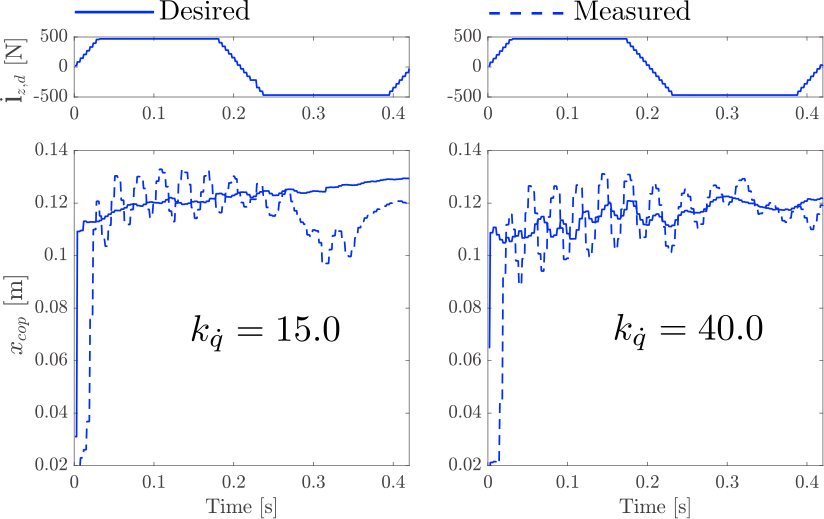
\includegraphics[width=0.9\textwidth]{STYLESTUFF/atlascop.png}
\caption{\ac{CoP} tracking during the two `bangs' of the vertical motion control law. In the left column, $k_{\dot{q}}=15.0$. In the right column, $k_{\dot{q}}=40.0$. For illustration of the `bangs', $\dotldz$ is graphed. }
\label{fig:atlascop}
\end{figure}

The approximate same magnitude of recoverable push on hardware for both setups is computed as follows. For an initial height of $z_0=1.10$ [m] and a maximum height of $\zmax=1.17$ [m], the average difference in recoverable ball height $\delta z_{ball}$ is:
\begin{equation}
	\delta z_{ball} = l_{rope} - \sqrt{l_{rope}^2-l_{ball}} = 6.12-\sqrt{6.12^2 - 2.79^2} = 0.673 \quad \text{[m]},
\end{equation}
where $l_{rope}$ is the length of the rope between the ceiling attachment point and the ball. The impulse applied on the robot is calculated as:
\begin{equation}
m_{ball}\dot{x}_{ball} = m_{ball}\sqrt{2g\delta z_{ball} } = 13.6\sqrt{2 \cdot 9.81 \cdot 0.673} = 49.4 \quad \text{[Ns]}.
\end{equation}
Normalizing the impulse, like with Valkyrie, results in a value of $i=\frac{49.4}{155.9}=0.317$ [m/s]. From the logging camera it is observed that the push duration is in the range $0.06-0.08$ [s].

\section{Discussion}
In this chapter, a simple control law is presented, that activates a bang-bang action if a predefined worst-case scenario is met. Using the bang-bang controller, the vertical \ac{CoM} dynamics are explicitly solvable and can be computed every tick. Also, hardware results are presented, which have not earlier been shown considering this topic. 

A difference between the related works in Section \ref{sec:relatedworksheight} is that most other existing control strategies use \ac{MPC}. With \ac{MPC} however, it all comes down to problem formulation. Caron \& Mallein present in \cite{caron2018balance} a method that generates capture trajectories based on the current \ac{CoM} position and velocity and the support polygon. The objective is to minimize height variations, which results in the robot to only use vertical \ac{CoM} motion if the desired \ac{ZMP} is placed on the polygon edge. Using this problem formulation though, the resulting capture trajectory is always under the assumption that the previously applied disturbance stopped disturbing. In the case of a push though, the increase in error is not an instant event and happens over time.

The control law in this chapter presents a different approach to the problem. Comparing with the method of Caron \& Mallein, which has a constraint on minimum and maximum vertical acceleration in the \ac{MPC} law, the bang-bang controller in this chapter can be seen as the extremum of what the \ac{MPC} would output. Therefore, the term `worst-case' is used to describe when the bang-bang law should be activated. This worst-case event is barely a tuning parameter and in this chapter considered when the proportionally controlled $\rcopd$ touches the polygon edge. An advantage of this formulation is that by choosing the worst-case with a safety margin, the control law always tries to exert the maximum allowed force to recover. This can result however in unnecessary height variations, which could be less the case in the \ac{MPC} law of Caron \& Mallein.

There are two test setups considered in this chapter for testing the controller on hardware while the robot is standing, which both test push recovery. An advantage of the test with the stick is that the force data on the load cell could be measured with an accuracy of $0.25$ \% at a record frequency of $100$ [Hz] \cite{iload}. However, many tests had to be conducted to obtain the results of the maximum recoverable pushes, as the person pushing the robot was not always capable of applying the exact same force. With the medicine ball tests, the maximum recoverable push could be found more easily and less tests were needed. However, no measurement data was available, and stretch in the rope, \ac{CoM} in the ball and release of the ball can all influence the impulse  applied on the robot.

Testing push recovery, Valkyrie and Atlas showed a similar behavior in simulation. In \ac{SCS}, a ground stiffness and damping is modeled, where the robot is in contact with the ground with $4$ ground contact points. Also, a joint torque damping is simulated. However, the differences in Atlas and Valkyrie and simulation are predominantly related to differences in the sizes and inertia of each limb.

On hardware however, larger differences were observed when comparing the responses of Valkyrie and Atlas. Valkyrie matched the simulation data with more accuracy, which could be a cause of the torque sensing of the series elastic actuators. However, while performing the test it is observed that Valkyrie is more sensitive for tuning of the maximum vertical acceleration, maximum jerk and for example foot polygon size used in the whole-body \ac{QP}. With careless tuning, Valkyrie could stand on its toes when recovering from a push, or the actuators could turn in a state of over-excitation which resulted in the need to restart the robot. Using Atlas, less care had to be taken for tuning and the robot performed well in all tests in terms of internal stability. The less accurate sensing and the stiction in the hydraulic system on Atlas could be a cause that the difference between hardware and simulation are larger.

To analyze the responses on hardware, on Valkyrie a phase plot of the horizontal \ac{CoM} state and different time responses are evaluated. The phase plots give insight in the ability of the robot to return to the desired steady-state configuration. The time-response plots show the behavior of momentum rates, joint pitch torque and \ac{CoP} and \ac{ICP} positions over time. However, no traditional system evaluations are conducted, such as a bode plot or other frequency analysis methods. A reason for this is that in the control method, the eigenvalue of the system is time-variant.

On most tests the improvement in recovery of the vertical motion control law versus the default control setup differs  from the difference in the \ac{CP} and the vertical force constraint capture points. Reasons for this could include numerical integration in simulation, unmodeled dynamics such as ground contact or a bug in the software.

Furthermore, the control strategy presented in this chapter is a \ac{2D} strategy. The third dimension is controlled with the $\rcopd$ orthogonal to the push direction, already existing in the control framework. When the robot is walking however, this \ac{2D} strategy does not always improve balance. Therefore, the control strategy presented in this chapter is extended in the next chapter for the use in \ac{3D}.



